\section{Verwendete Tools}

Für die Implementierung des gewünschten Systems muss ein Framework verwendet werden, in dem alle diese gegebenen Anforderungen erfüllt werden können. Dieses selbst zu implementieren würde sowohl nicht dem Rahmen einer Bachelorarbeit entsprechen als auch voraussichtlich nicht die Möglichkeiten bestehender Werkzeuge erreichen, weshalb eine vorgefertigte Lösung verwendet wird.

Das Robot Operating System 2 von Open Robotics \cite{ros}, welches dafür konzipiert wurde, eine Kommunikation zwischen Robotern und anderen Computern in nahezu Echtzeit zu ermöglichen, ist als Framework für diese Art von System geeignet. Dieses erfüllt die Anforderung an die Skalier- und Erweiterbarkeit, da es sowohl über einen zentralen als auch verteilte Knoten betrieben werden kann und daher mit dem System wächst, ohne einen Engpass darzustellen. Auch ist es ein Open Source-Framework und verfügt über eine öffentlich zugängliche Dokumentation, sodass in dieser Hinsicht die Erweiterung durch Dritte keinerlei Probleme darstellen sollte. Es kann unter Windows, Ubuntu Linux, macOS und RHEL installiert und betrieben werden und unterstützt nativ die Programmierung von Knoten in den Sprachen Python und C++.

Ein Netzwerk in ROS ist um eine Mehrzahl von Knoten herum aufgebaut. Diese können einzelne Roboter, Geräte oder Prozesse innerhalb des System-Netzwerks darstellen. ROS ermöglicht es, zwischen Knoten verschiedene Dateninhalte über sogenannte Topics, Services und Actions zu teilen. Topics stellen dabei eine Ein-Wege-Kommunikation auf einem ständig offenen Kanal dar. Knoten können an Topics Nachrichten senden und von diesen solche empfangen, wobei es unerheblich ist, wie viele Knoten Nachrichten von einem Topic lesen. Dadurch können in Echtzeit Statusmeldungen und sich kontinuierlich ändernde Daten geteilt werden.

Services dagegen stellen eine Zwei-Wege-Kommunikation dar, bei der ein Client-Knoten einen bestimmten Service von einem Server-Knoten anfragt. Knoten, welche als solche Service Server konfiguriert wurden, senden Nachrichten nur dann, wenn über einen Request des Service Clients diese angefordert werden. Dies verhindert, dass selten benötigte oder sich nur selten ändernde Daten unnötige Bandbreite belegen, indem sie kontinuierlich gesendet werden müssen. Auch können so Anweisungen von einem Knoten an einen anderen gegeben werden.

Actions sind eine erweiterte Form von Services, bei denen davon ausgegangen wird, dass die Beantwortung einer Anfrage eine gewisse Zeit in Anspruch nimmt. Nach einer Bestätigung einer Anfrage sendet daher der Server-Knoten auf einem Topic Statusmeldungen, um den Client-Knoten über den Fortschritt der Anweisung zu informieren, bis die Anfrage abschließend bearbeitet wurde. Dies wird vor allem dann benutzt, wenn cyber-physikalische Systeme angesprochen werden, die andauernde Aktionen ausführen. 

Durch diese Kommunikationswege ist es für das System möglich, sowohl für die Kommunikation zu Geräten als auch zu Schnittstellen der Benutzeroberfläche dieselbe Middleware zu verwenden und den Nachrichtenversand an die Anforderungen anzupassen. Dadurch kann auch nativ ein Multi-User Konzept für die Eingabe von Nutzeranweisungen realisiert werden, in welchem jeder Zugang einen eigenen Knoten darstellt, welcher über entsprechende Topics mit dem System kommuniziert. Alle Nachrichten können in ROS standardmäßig auf der Kommunikationsebene verschlüsselt und authentifiziert werden, sodass der Nutzerzugang über gesicherte Schnittstellen sicher gestellt werden kann.

Zur Programmierung der Knoten wird in diesem Projekt die Programmiersprache Python verwendet. Eine Verwendung von C++ oder anderer Sprachen, welche durch Einbindung von Drittpartei-Libraries unterstützt werden könnten, könnte unter Umständen die Ausführung des Systems beschleunigen. Da diese jedoch im Vergleich zu Netzwerk-Latenzen und Datenbank-Zugriffsgeschwindigkeiten vernachlässigbar klein sind, stellt Python als weit verbreitete und leicht zu erlernende Sprache durch die Erleichterung der Erweiterbarkeit durch Dritte die bessere Wahl dar.

Die Datenbanken werden in der Implementierung mithilfe von SQLite3 erstellt, einer Library zu Erstellung von ressourcenschonenden Datenbanken. Es basiert auf der SQL-Sprache, welche die Basis für die meisten Datenbanksysteme ist. SQLite bietet die Möglichkeit, Befehle direkt in Python-Programmen zu verwenden, sodass keine externe Software zur Übersetzung nötig ist.


\FloatBarrier
\section{Systemarchitektur}

Die Umsetzung der Systemarchitektur wird mithilfe voneinander unabhängiger ROS-Knoten umgesetzt, welche in einer gemeinsamen Umgebung kompiliert werden, allerdings auch als einzelne Pakete ausgeführt werden können. Jeder Knoten besteht dabei aus einem Kern-Knoten, welcher zuerst initialisiert wird und den Ansprechpartner für andere Knoten darstellt. Dazu verfügen die einzelnen Kern-Knoten zum Teil über sekundäre Knoten, auf die bestimmte Aufgaben ausgelagert werden, um eine Parallelisierung von Abläufen zu ermöglichen. Diese werden in den einzelnen Knoten-Beschreibungen näher erläutert.

Die Implementierung unterscheidet sich in zwei Punkten von dem Gesamtkonzept und erfüllt bisher nicht alle Ansprüche des Systems, um der Arbeit einen angemessenen Umfang zu geben. Zum einen wird dadurch, dass von einer später zu entwickelnden Nutzerschnittstelle ausgegangen wird, stattdessen eine Befehlseingabe per Konsole zur Verfügung gestellt. Diese ermöglicht, alle implementierten Funktionen des Systems direkt zu nutzen, ohne eine dedizierte Plattform bereitstellen zu müssen. Dazu sind einige Nutzereingaben, die über das Ziel der Implementierung hinausgehen, implementiert worden, um die Entwicklung und das Testen des Systems zu vereinfachen.

Da die explizite Implementierung von Navigationsstrategien von Robotern nicht Ziel dieser Arbeit ist, verfügt die hier vorgestellte Lösung zum anderen auch über keinen Navigationsknoten oder dazugehörige Services. Insbesondere stehen keine verwendbaren Navigationsbefehle in der Datenbank des Planungsknotens zur Verfügung. Auch ist auf eine Umsetzung der Warteschlange für auszuführende Pläne verzichtet worden, da durch den nicht implementierten Navigationsknoten die Abfrage von diesen nicht erfolgt.

Die Kommunikation zwischen den Knoten wird über sogenannte Interfaces definiert, welche einen Rahmen für die jeweiligen Nachrichten bieten. In dieser Implementierung werden nur eigene Interfaces für Services verwendet, welche dementsprechend die Dateiendung '.srv' besitzen. Jedes dieser Interfaces kann eine Mehrzahl an Argumenten unter einem Alias und einer Spezifikation des verwendeten Datentyps für jeweils den Service-Aufruf und die Antwort aufnehmen.

Diese Interfaces sind hier nach dem jeweiligen Verwendungszweck zusammengefasst. Services, welche sich mit Gegenständen befassen, verwenden das Interface 'Item.srv', solche für Szenarien 'Goal.srv', jene für Pläne 'Plan.srv' und diejenigen, die sich mit dem Anlegen von Datenbanken befassen, 'MakeDB.srv'. Die jeweiligen Argumente der Interfaces samt Datentyp und Verwendungszweck sind in der folgenden Tabelle aufgeführt.

\begin{table}[h]
\begin{center}
\begin{tabular}{| c | c | c | l |}
  \hline
  Interface & Datentyp & Argument & Verwendungszweck \\
  \hline
  \hline
  Item.srv   & int32   & id            & ID-Nummer eines bestimmten Gegenstandes\\
             & string  & item\_kind    & Art eines Gegenstandes\\
             & string  & position      & Position eines Gegenstandes in 2D-Ebene\\
             & int32   & begin\_date   & Anfangszeit einer Reservierung\\
             & int32   & end\_date     & Abschlusszeit einer Reservierung\\
             & bool    & ack           & Antwort - Bestätigung eines Aufgabeneingangs\\
             & int32[] & reserved\_ids & Antwort - ID-Nummern reservierter Gegenstände\\
  \hline
  \hline
  Goal.srv   & int32   & goal\_id      & ID-Nummer eines bestimmten Szenarios\\
             & string  & goal\_desc    & Beschreibung eines Szenarios\\
             & string  & goal\_nav     & Navigationsbefehle des Szenarios\\
             & bool    & ack           & Antwort - Bestätigung eines Aufgabeneingangs\\
  \hline
  \hline
  Plan.srv   & int32   & id            & ID-Nummer eines bestimmten Plans\\
             & int32   & goal\_id      & ID-Nummer des angewendeten Szenarios\\
             & string  & items         & Liste der verwendeten Gegenstände\\
             & int32   & begin\_time   & Anfangszeit eines Plans\\
             & int32   & end\_time     & Abschlusszeit eines Plans\\
             & bool    & ack           & Antwort - Bestätigung eines Aufgabeneingangs\\
  \hline
  \hline
  MakeDB.srv & string  & db\_name      & Name der anzulegenden Datenbank\\
             & bool    & ack           & Antwort - Bestätigung eines Aufgabeneingangs\\
  \hline
  \hline
  String.msg & string  & user\_info    & Senden der Systemmitteilungen an Nutzer\\
  \hline
\end{tabular}
\caption{Verwendete Interfaces}
\end{center}
\end{table}

Das Topic 'user\_information', an welches Knoten für Nutzer relevante Informationen über ihre ausgeführten Aufgaben teilen, benötigt kein eigenes Interface. Hier kann das in ROS2 vorhandene String-Format verwendet werden, da in dieser Implementierung nur Textzeilen übertragen werden.


\FloatBarrier
\section{User Interface}

Der User Interface-Knoten ist aus drei ROS-Knoten aufgebaut: dem 'NodeUICore', den 'NodeUICommunicator' und dem 'NodeUIOutput'. Der NodeUICore nimmt Nutzereingaben entgegen und gibt diese an den NodeUICommunicator weiter. Dieser übersetzt Nutzereingaben in Service-Anfragen an andere Knoten. NodeUIOutput nimmt die auf dem Topic 'user\_interface' geteilten Nachrichten und gibt sie in einem eigenen Konsolen-Fenster aus.

NodeUICore initialisiert beim Start auch NodeUICommunicator, um an die Planungs- und Logistikknoten die Anweisung zu übermitteln, sich mit den jeweiligen Datenbanken zu verbinden. Ansonsten verfügt die Klasse nur über ein Attribut 'service\_choice', welches die Eingabe zur Weitergabe beinhaltet. Nach der Initialisierung ruft der Knoten die Funktion 'select\_service()' auf, mittels der dem Nutzer die wählbaren Optionen angezeigt werden und eine Auswahl per Konsoleneingabe angenommen wird. Diese Auswahl wird über das Attribut service\_choice dann an NodeUICommunicator per Funktionsaufruf weitergegeben. Die Ausführung von select\_service() kann über einen Befehl 'close\_ui' unterbrochen werden, wodurch der Knoten anschließend terminiert.

\begin{table}[h]
\begin{center}
\begin{tabular}{| c | l | c |}
  \hline
  Nutzereingabe & Aktion & Ausführender Knoten\\
  \hline
  \hline
  show\_item    & zeigt einen Gegenstand an           & Logistik \\
  show\_goal    & zeigt ein Szenario an               & Planung  \\
  show\_plan    & zeigt einen Plan an                 & Planung  \\
  create\_item  & erstellt einen neuen Gegenstand     & Logistik \\
  create\_goal  & erstellt ein neues Szenario         & Planung  \\
  create\_plan  & erstellt einen neuen Plan           & Planung  \\
  edit\_item    & ändert die Daten eines Gegenstandes & Logistik \\
  edit\_goal    & ändert die Daten eines Szenarios    & Planung  \\
  edit\_plan    & ändert die Daten eines Plans        & Planung  \\
  delete\_item  & löscht einen Gegenstand             & Logistik \\
  delete\_goal  & löscht ein Szenario                 & Planung  \\
  delete\_plan  & löscht einen Plan                   & Planung  \\
  close\_ui     & schließt den User Interface-Knoten  & ---      \\
  \hline
\end{tabular}
\caption{Verfügbare Befehle}
\end{center}
\end{table}

Bei der Initialisierung von NodeUICommunicator werden im Gegensatz zum Kern-Knoten keinerlei Handlungen ausgeführt. Der Knoten wird stattdessen nur zur Ausführung einzelner Funktionsaufrufe verwendet, nach denen der Knoten wieder geschlossen wird. Der Aufruf findet über die oben beschriebene Funktion select\_service von NodeUICore statt. Jede der Funktionen fügt die gegebenenfalls erforderlichen Konsoleneingaben zu einer Service Request zusammen, um diese Request dann an den Knoten zu senden, der in der Tabelle 'Verfügbare Befehle' angegeben ist.

\begin{figure}
\begin{center}
\begin{tikzpicture}
\begin{umlpackage}{User Interface}
\umlclass{NodeUICore}
{service\_choice : string \\
 node\_comm : Node = NodeUICommunicator()}
{select\_service() : void}

\umlclass[x=8, y=-5]{NodeUICommunicator}
{input : string}
{make\_plan\_db() : MakeDB.Request()\\
 show\_item(input) : Item.Request()\\
 show\_goal(input) : Goal.Request()\\
 show\_plan(input) : Plan.Request()\\
 create\_item(input) : Item.Request()\\
 create\_goal(input) : Goal.Request()\\
 create\_plan(input) : Plan.Request()\\
 edit\_item(input) : Item.Request()\\
 edit\_goal(input) : Goal.Request()\\
 edit\_plan(input) : Plan.Request()\\
 delete\_item(input) : Item.Request()\\
 delete\_goal(input) : Goal.Request()\\
 delete\_plan(input) : Plan.Request()\\
 close\_ui() : void
}

\umlclass[x=0, y=-5]{NodeUIOutput}
{subscription : create\_subscription() \\
 msg : string}
{listener\_callback(msg) : void}

\umluniassoc[geometry = -|, arg1=select\_service(), align1=left]
{NodeUICore}{NodeUICommunicator}
\end{umlpackage}
\end{tikzpicture}
\caption{User Interface-Knoten: Klassendiagramm}
\end{center}
\end{figure}

Zuletzt liegt der Knoten NodeUIOutput im Paket, welcher keine Interaktion mit den anderen beiden Knoten ausführt. Die einzige Aufgabe des Knotens ist, Nachrichten an das Topic 'user\_information' zu empfangen und auf einer Konsole auszugeben. Dementsprechend verfügt der Knoten auch nur über die Funktion 'listener\_callback(msg)', welche die empfangenen Nachrichten mit einem Zeitstempel druckt.


\FloatBarrier
\section{Planung}

Das Paket des Planungsknotens ist ähnlich dem vorangehenden User Interface aufgebaut, auch hier gibt es einen Kern- und einen Kommunikationsknoten, 'NodePlanCore' und 'NodePlanCommunicator' genannt. NodePlanCore nimmt hier aber Service Requests anderer Knoten entgegen, um diese zu bearbeiten. Hierfür besteht auch eine Verbindung zu der Datenbank des Planungsknotens, um SQL-Befehle an diese zu geben.

NodePlanCore dient als Service Server für eine Vielzahl von Funktionen, deren Verbindungsschnittstellen bei der Initialisierung geöffnet werden. All diese Services rufen eine eigene Rückruffunktion mit dem Namen 'callback\_(Name des Service)' auf, welche der Request mit den übermittelten Parametern entgegennehmen und nach Abschluss auf diese antworten. Zur Umsetzung des Services wird dann eine Datenbank-Funktion mit dem Namen 'db\_(Name des Service)' aufgerufen, welche die Parameter der Request erhält und die entsprechende Aktion ausführt. Nach Abschluss der Datenbank-Funktion sendet die Rückruffunktion dann eine Bestätigung des Services zurück und sendet zusätzlich eine Nachricht an das Topic 'user\_information', in der die gerade vorgenommene Aktion beschrieben ist.

\begin{table}[h]
\begin{center}
\begin{tabular}{| c | c | l |}
  \hline
  Service        & Interface & Parameter                                         \\
  \hline
  \hline
  make\_plan\_db & MakeDB    & ---                                               \\
  show\_goal     & Goal      & goal\_id                                          \\
  show\_plan     & Plan      & plan\_id                                          \\
  create\_goal   & Goal      & goal\_desc                                        \\
  create\_plan   & Plan      & goal\_id, items, begin\_time, end\_time           \\
  edit\_goal     & Goal      & goal\_desc, goal\_id                              \\
  edit\_plan     & Plan      & plan\_id, goal\_id, items, begin\_time, end\_time \\
  delete\_goal   & Goal      & goal\_id                                          \\
  delete\_plan   & Plan      & plan\_id                                          \\
  \hline
\end{tabular}
\caption{Planungsknoten: Ausführbare Services}
\end{center}
\end{table}

Die Datenbank-Funktionen der jeweiligen Services fügen aus den weitergegebenen Parametern der Request und einem generischen SQL-Befehl die Anweisung an die Datenbank zusammen und lassen diese ausführen. Daten der verwendeten Tabelle, die von der Rückruffunktion erwartet werden, werden in dieser von der Datenbank-Funktion ausgelesen. Dieses Schema trifft einzig nicht auf die Funktion 'callback\_create\_plan' zu, da diese zusätzlich zu dem Datenbank-Aufruf auch einen Service Request an den Logistik-Knoten senden muss, um die benötigten Gegenstände zu reservieren. Hierzu wird bei Funktionsaufruf erst eine Anfrage an den Logistik-Knoten mit den benötigen Gegenstandsarten gesendet, um festzustellen, ob der anzulegende Plan umsetzbar ist. Im Falle einer positiven Response wird dann die ursprüngliche Request, welche um die ID-Nummern der reservierten Gegenstände erweitert wurde, an die Datenbank-Funktion weitergegeben.

\begin{figure}
\begin{center}
\begin{tikzpicture}
\begin{umlpackage}{Planung}
\umlclass{NodePlanCore}
{conn : sqlite3.connect(self.db\_file) \\
 msg : string \\
 node\_comm : Node = NodePlanCommunicator()\\
 srv\_$*$ : create\_service()
 publisher\_ : create\_publisher()}
{callback\_$*$(request, response) : response \\
 db\_$*$(request) : Datenbank-Antwort}

\umlclass[x=0, y=-5]{NodePlanCommunicator}
{}
{reserve\_item(item\_kind, begin\_date, end\_date) : Item.Request()}

\umluniassoc[arg1=create\_plan()]
{NodePlanCore}{NodePlanCommunicator}
\end{umlpackage}
\end{tikzpicture}
\caption{Planungsknoten: Klassendiagramm}
\end{center}
\end{figure}

Die Datenbank selbst ist in drei Tabellen unterteilt: 'goals', 'rooms' und 'goal\_planning'. Die erste Tabelle nimmt die einzelnen Szenarien, in der Implementierung ebenfalls als 'goals' bezeichnet, auf und speichert neben der jeweiligen ID-Nummer auch die Beschreibung des Szenarios und die benötigten Gegenstände und Räume. Dazu soll die Tabelle auch die Navigationsanweisungen enthalten, mit denen der Plan ausgeführt werden kann. Da diese aber noch nicht erstellt sind, wird derweil ein Platzhalter verwendet.

'rooms' umfasst dagegen die verfügbaren Räume, sodass in der Planung freie Räume gesucht werden können. Die Tabelle goal\_planning verweist auf die erste und zweite Tabelle, versieht die Szenarien jedoch mit konkreten ID-Nummern für die Gegenstände und Räume und einer Zeitspanne zur Ausführung. Die Zeitspanne ist dabei in UNIX Time angegeben, da diese von nahezu allen Maschinen gelesen und verwendet werden kann. Für jede der drei Tabellen ist unten jeweils ein Beispiel angegeben.

\begin{table}[h]
\begin{center}
\begin{tabular}{| c | c | c | c | c |}
  \hline
  \textbf{id} & \textbf{goal}     & \textbf{instructions}    & \textbf{items}    & \textbf{room\_kind}\\
  \hline
  \hline
  1           & Set up a meeting! & [Navigationsdaten] & table chair chair & conference room    \\
  \hline
\end{tabular}
\caption{Planungsknoten Datenbank, 'goals'-Tabelle}
\end{center}
\begin{center}
\begin{tabular}{| c | c |}
  \hline
  \textbf{id} & \textbf{room\_kind} \\
  \hline
  \hline
  1           & conference room     \\
  \hline
\end{tabular}
\caption{Planungsknoten Datenbank, 'rooms'-Tabelle}
\end{center}
\begin{center}
\begin{tabular}{| c | c | c | c | c | c |}
  \hline
  \textbf{id} & \textbf{goal\_id} & \textbf{room\_id} & \textbf{item\_ids} & \textbf{begin\_date} & \textbf{end\_date} \\
  \hline
  \hline
  1           & 1                 & 1                 & 1 2 3              & 1645848800           & 1645872600         \\
  \hline
\end{tabular}
\caption{Planungsknoten Datenbank, 'goal\_planning'-Tabelle}
\end{center}
\end{table}


\FloatBarrier
\section{Logistik}

Der Logistikknoten verwaltet die Datenbank und bearbeitet Service Requests, sendet aber selbst keine Anfragen an andere Knoten. Dementsprechend verfügt das Paket auch nur über den Kern-Knoten 'NodeLogCore'. Genauso wie NodePlanCore bietet auch dieser Service Schnittstellen an und stellt die Verbindung zu der Datenbank des Knotens her. Ebenfalls stehen für jeden Service jeweils eine Rückruf- und eine Datenbank-Funktion zur Verfügung.

\begin{table}[h]
\begin{center}
\begin{tabular}{| c | c | l |}
  \hline
  Service        & Interface & Parameter                                         \\
  \hline
  \hline
  make\_log\_db  & MakeDB    & ---                                               \\
  show\_item     & Item      & item\_id                                          \\
  create\_item   & Item      & item\_kind, position                              \\
  edit\_item     & Item      & id, item\_kind                                    \\
  delete\_item   & Item      & item\_id                                          \\
  \hline
\end{tabular}
\caption{Logistik-Knoten: Ausführbare Services}
\end{center}
\end{table}

Von besonderer Bedeutung ist der Service 'reserve\_item'. Der Parameter 'items' nimmt eine Liste von Gegenstandsarten entgegen, bei der geprüft werden muss, ob darauf passende Gegenstände verfügbar sind. Dazu kann kein einzelner SQL-Befehl gegeben werden. Aus der Tabelle 'item\_logistics' der Datenbank wird daher zunächst für jede angefragten Art eine Liste der verfügbaren Gegenstände anhand bestehender Reservierungen generiert. Falls für jede Art der Gegenstände genügend in der Liste vorhanden sind, werden in einem zweiten Datenbankzugriff die entsprechenden Gegenstände reserviert und eine Aufzählung der ID-Nummern der verwendeten Gegenstände an den Planungsknoten zurückgegeben.

\begin{figure}
\begin{center}
\begin{tikzpicture}
\begin{umlpackage}{Logistik}
\umlclass{NodeLogCore}
{conn : sqlite3.connect(self.db\_file) \\
 msg : string \\
 srv\_$*$ : create\_service()
 publisher\_ : create\_publisher()}
{callback\_$*$(request, response) : response \\
 db\_$*$(request) : Datenbank-Antwort}
\end{umlpackage}
\end{tikzpicture}
\caption{Logistik-Knoten: Klassendiagramm}
\end{center}
\end{figure}


Die Datenbank des Logistik-Knotens besteht aus den Tabellen 'items' und 'item\_logistics'. Die erste Tabelle fasst die ID-Nummer jedes einzelnen Gegenstands, dessen Position im 2D-Raum sowie die Art des Gegenstands. Die Position ist für die geplante Navigation wichtig, da so die Gegenstände gefunden werden können, und wird in einem Integer-Array gespeichert, das die x und y-Werte auf der Navigationskarte hält. Die Art des Gegenstands ist dagegen für den Planungsknoten für Bedeutung, da über diesen Eintrag nach Gegenständen zur Umsetzung von Szenarien gesucht wird. Die Tabelle 'item\_logistics' dient dazu, Reservierungen der Gegenstände zu speichern. Dabei spiegelt jeder Eintrag eine Reservierung wider, die neben der ID-Nummer des Gegenstands auch die Zeitspanne angibt, wann dieser Gegenstand nicht verfügbar ist.

\begin{table}[h]
\begin{center}
\begin{tabular}{| c | c | c |}
  \hline
  \textbf{id} & \textbf{position} & \textbf{item\_kind} \\
  \hline
  \hline
  1           & [3 4]             & table               \\
  2           & [5 6]             & chair               \\
  3           & [1 1]             & chair               \\
  \hline
\end{tabular}
\caption{Logistik-Knoten Datenbank, 'items'-Tabelle}
\end{center}
\end{table}

\begin{table}[h]
\begin{center}
\begin{tabular}{| c | c | c | c |}
  \hline
  \textbf{id} & \textbf{item\_id} & \textbf{begin\_date} & \textbf{end\_date} \\
  \hline
  \hline
  1           & 1                 & 1645848800           & 1645872600         \\
  2           & 2                 & 1645848800           & 1645872600         \\
  3           & 3                 & 1645848800           & 1645872600         \\

  \hline
\end{tabular}
\caption{Logistik-Knoten Datenbank, 'item\_logistics'-Tabelle}
\end{center}
\end{table}

\FloatBarrier
\section{Evaluation}

Um den Betrieb des Systems zu überprüfen, wird ein einfacher Funktionstest durchgeführt. Da es sich hier um ein Prototypen-System handelt, wird keine umfassende quantitative Evaluation vorgenommen. Dementsprechend kann auch kein Anspruch auf Betriebsbereitschaft in einem Skills Lab gestellt werden.

Der Funktionsumfang des Systems umfasst in seinem derzeitigen Zustand das Anlegen, verändern und löschen von Gegenständen, Szenarien und Plänen. Da die Programmierung des Systems in der englischen Sprache erfolgt ist, werden diese in den Systemanzeigen als 'item', 'goal' und 'plan' bezeichnet.

Um die Funktionen zu überprüfen, wird eine Reihe von Eingaben getätigt, welche alle Funktionen abdecken. Da die Daten der Gegenstände, Szenarien und Pläne aufeinander aufbauen, werden sie auch in dieser Reihenfolge überprüft. Dabei werden für alle drei Fälle zunächst eine Reihe Einträge angelegt, daraufhin wird einer von diesen verändert und ein zweiter gelöscht. Danach wird über ein Zugriff auf die Datenbank-Tabelle festgestellt, ob die Eingaben korrekt bearbeitet wurden.

Das Ziel der Eingaben wird sein, ein Meeting anzulegen und vorzubereiten. Dazu werden als Gegenstände zwei Stühle und ein Tisch benötigt. Das Meeting soll am ersten Januar 2023 um 12 Uhr Mittags stattfinden, also zum Zeitpunkt '1672570800' in Unix-Zeit, und eine Stunde dauern. Es soll im Konferenzraum stattfinden, der die Raumnummer 1 trägt. Es wird dafür mit dem System im Ausgangszustand begonnen, bei dem keine der drei Datenbanken vorliegt. Einzig die Tabelle der Räume ist vorher mit einem Raum 'meeting room' initialisiert. Da die Raumverteilung in einem Skills Lab als gegeben angesehen wird, gibt es für diese keine Nutzereingabe.

Im ersten Schritt werden hierfür die Gegenstände 'chair', 'table', 'table' und 'lamp' angelegt. Dies geschieht über die Konsoleneingabe, wie sie in der folgenden Bildschirmaufnahme exemplarisch abgebildet wird. Für die Positionen werden willkürliche Werte eingetragen, da diese ohne Vorhandensein des Navigationsknotens bedeutungslos sind. Im Anschluss wird der dritte Eintrag gelöscht, da nur ein Tisch benötigt wird. Dazu wird der Eintrag der Lampe zu einem zweiten Stuhl geändert. In der Bildschirmaufnahme ist der Zustand der Tabelle nach anlegen aller vier Einträge und nach Löschung des dritten und Änderung des vierten Gegenstands zu sehen.

\begin{figure}[h]
\centering
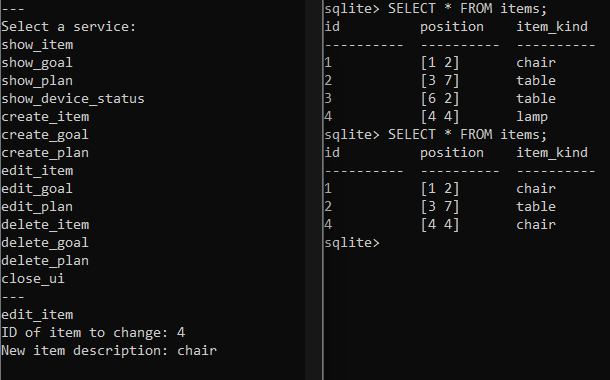
\includegraphics[width=(0.7\textwidth)]{Bilder/Eval1.png}
\caption{Evaluation: 'items' Datenbank}
\end{figure}

Im zweiten Schritt wird das Szenario angelegt. Hier werden zwei Szenarien angelegt. Das erste trägt die Beschreibung \dq set up a meeting \dq, hat als benötigte Gegenstände einen Tisch eingetragen und findet im Konferenzraum statt. Das zweite Szenario findet ebenfalls im Konferenzraum statt, trägt die Beschreibung \dq another meeting \dq und benötigt neben dem Tisch auch drei Stühle. Für diesen Test wird das zweite Szenario wieder gelöscht, und das erste wird so verändert, dass zwei Stühle zusätzlich zum Tisch benötigt werden.

\begin{figure}[h]
\centering
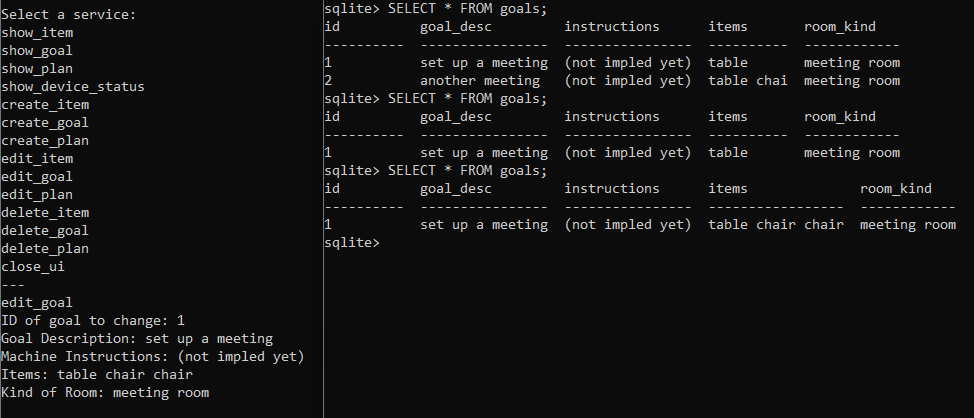
\includegraphics[width=(\textwidth)]{Bilder/Eval2.png}
\caption{Evaluation: 'goals' Datenbank}
\end{figure}

Im dritten und letzten Schritt wird das Szenario dann als Plan umgesetzt. Das aus dem letzten Schritt verbliebene Szenario besitzt die ID-Nummer 1, daher wird diese eingetragen. Statt der richtigen Uhrzeit wird aber Mitternacht des ersten Januar als Start-Zeitpunkt eingetragen und dementsprechend 1 Uhr nachts als End-Zeitpunkt. Ein zweiter Eintrag, der dasselbe Szenario umsetzen soll, erhält als Zeitpunkte 16, um sie visuell vom ersten Eintrag abzusetzen. Dieser zweiter Eintrag wird daraufhin wieder gelöscht, und die korrekte Zeiten 1672570800 und 1672574400, welche 12 und 13 Uhr mittags darstellen, werden im ersten Eintrag eingetragen. Dadurch liegt, wie in der Bildschirmaufnahme sichtbar, nur noch der korrekte Plan in der Datenbank.

\begin{figure}[h]
\centering
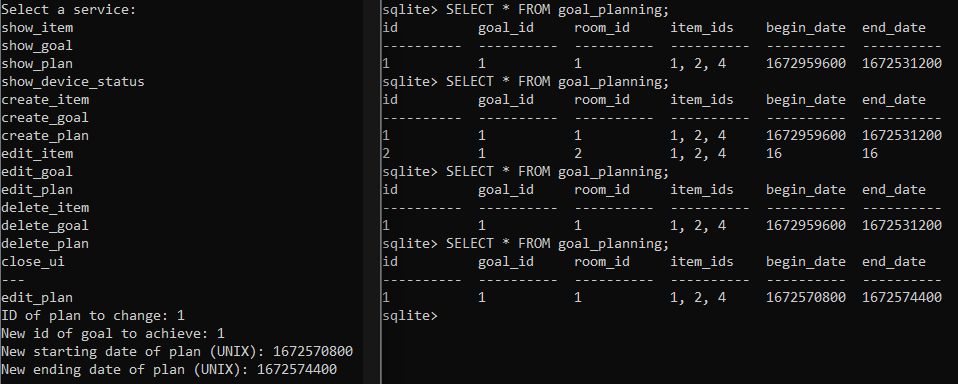
\includegraphics[width=(\textwidth)]{Bilder/Eval3.png}
\caption{Evaluation: 'goal\_planning' Datenbank}
\end{figure}

Durch das Anlegen eines Plans sollen auch Gegenstände reserviert werden, was wie im Ausschnitt unten erkennbar erfolgt. Der Eintrag 'item\_id' stimmt mit den im ersten Schritt angelegten Gegenständen überein, und die Zeiten sind ebenfalls der Änderung im dritten Schritt entsprechend. Demnach werden alle Funktionen wie erwartet ausgeführt.

\begin{figure}[h]
\centering
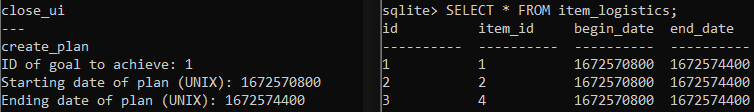
\includegraphics[width=(\textwidth)]{Bilder/Eval4.png}
\caption{Evaluation: 'item\_logistics' Datenbank}
\end{figure}